\documentclass[11pt]{amsart}
\usepackage[T1]{fontenc}
\usepackage{lmodern}
\input{glyphtounicode-cmex}
\pdfgentounicode=1
\usepackage[margin=1in]{geometry}
\usepackage{amsmath,amssymb,amsthm,mathtools}
\usepackage{microtype}
\AtBeginDocument{\begingroup\fontencoding{OT1}\footnotesize\selectfont\endgroup}
\usepackage{enumitem}
\usepackage{float}
\usepackage{tikz}
\usetikzlibrary{arrows.meta,patterns,calc}
\usepackage[colorlinks=true,linkcolor=blue!45!black,citecolor=blue!45!black,urlcolor=blue!45!black]{hyperref}
\usepackage[capitalise,noabbrev]{cleveref}
\newtheorem{theorem}{Theorem}[section]
\newtheorem{proposition}[theorem]{Proposition}
\newtheorem{lemma}[theorem]{Lemma}
\newtheorem{corollary}[theorem]{Corollary}
\theoremstyle{definition}
\newtheorem{definition}[theorem]{Definition}
\theoremstyle{remark}
\newtheorem{remark}[theorem]{Remark}
\newtheorem*{maintheorem}{Theorem A}
\numberwithin{equation}{section}
\newcommand{\R}{\mathbb R}
\newcommand{\N}{\mathbb N}
\newcommand{\II}{\mathrm{II}}
\newcommand{\dd}{\,\mathrm d}
\newcommand{\pd}{\partial}
\newcommand{\norm}[1]{\left\lVert#1\right\rVert}
\newcommand{\abs}[1]{\left\lvert#1\right\rvert}
\DeclareMathOperator{\supp}{supp}
\DeclareMathOperator{\diag}{diag}
\title[A smooth metric with no local isometric immersion]{A Smooth Metric with No Local Isometric Immersion into Three-Space}
\author{OpenAI}
\date{September 24, 2026}
\hypersetup{
  pdftitle={A Smooth Metric with No Local Isometric Immersion into Three-Space},
  pdfauthor={OpenAI},
  pdfsubject={Smooth local isometric realization of Riemannian surfaces}
}
\begin{document}
\begin{abstract}
We construct a smooth positive-definite Riemannian metric on
\((-1,1)^2\) that agrees with the Euclidean metric to every order at
the origin, yet no neighborhood of the origin admits a smooth
isometric immersion into Euclidean three-space. This gives a negative
answer to the unrestricted smooth local isometric realization problem
for surfaces.
\end{abstract}
\maketitle

\section{Introduction}

The local isometric realization problem asks whether a Riemannian
surface \((\Sigma,g)\) can, near each point, be realized as a smooth
surface in Euclidean three-space. In local coordinates this means
finding a smooth map \(F\) with
\[
\langle \partial_iF,\partial_jF\rangle=g_{ij},
\qquad i,j\in\{1,2\}.
\]
Positive definiteness of \(g\) then forces \(\operatorname{rank}dF=2\).
The unrestricted smooth question is part of Yau's discussion of
isometric embedding~\cite[p.~236]{Yau2000} and is formulated explicitly
in Ghomi's survey~\cite[Section~1.5, Problem~1.9]{Ghomi2019}.
We give a negative answer to this local three-dimensional problem.

\begin{maintheorem}
There is a \(C^\infty\) positive definite Riemannian metric \(g\) on
\((-1,1)^2\) such that no open neighborhood \(U\) of the origin admits a
\(C^\infty\) isometric immersion
\[
F:(U,g)\longrightarrow\R^3.
\]
In particular, no such neighborhood admits a smooth isometric embedding.
\end{maintheorem}

A smooth isometric immersion is an embedding after restriction to a
sufficiently small neighborhood of any point. Thus the two local
formulations have the same existence content. No completeness or
topological assumption is involved in Theorem~A.
The metric can moreover be chosen to have the same full Taylor jet
at the origin as the Euclidean metric; see \Cref{cor:flat-jet}.
Thus smooth local realizability is not determined by that jet.

\subsection*{Curvature and regularity}
The analytic local problem is settled by the classical Janet--Cartan
theorem~\cite{Janet1926,Cartan1927}. For smooth metrics, nonzero
Gaussian curvature leads to elliptic or hyperbolic equations and
smooth local existence; zeros of curvature introduce degeneracy
and changes of type. Lin's foundational work treated nonnegative
curvature and a clean change of sign with finite differentiability
estimates~\cite{Lin1985,Lin1986}. Here a clean change of sign means
\(K(p)=0\) and \(dK(p)\ne0\). Smooth local existence under
this condition was established by Nakamura and Maeda~\cite{NakamuraMaeda1989};
see also the regularity comparison in \cite[p.~320]{NY2008}.
More complicated zero sets have been treated under finite-order
and geometric restrictions, including transverse curves and
cusps~\cite[Theorem~1.1]{HanKhuri2010}\cite[Theorem~1.1]{Lin2015}.

The regularity distinction is essential. Existence at every finite
differentiability order, on neighborhoods allowed to shrink with
that order, does not by itself give one smooth map on a fixed
neighborhood. At the other end of the scale, Nash--Kuiper
flexibility gives \(C^1\) local isometric realizations in
three-space~\cite{Nash1954,Kuiper1955}. That regularity does not
impose the second-order compatibility used for smooth immersions.
Pogorelov constructed a \(C^{2,1}\) metric with no local \(C^2\)
realization~\cite[paragraph~7]{Pogorelov1971}.
The published refinement by Nadirashvili and Yuan achieves
\(K\ge0\) with the same input and output
regularities~\cite[Theorem~1.1]{NY2008}.
In Theorem~A, positive definiteness refers to the metric, not its
curvature: the construction uses both signs of curvature.
It does not settle the smooth local-realizability problem under
either sign restriction \(K\ge0\) or \(K\le0\).

An earlier preprint of Nadirashvili and Yuan~\cite[Theorem~1.1]{NY2002}
states a stronger
counterexample: a smooth metric with \(K\le0\) and no \(C^3\)
isometric embedding on any neighborhood of the distinguished
point. Their later published paper, however, explicitly leaves
the arbitrary smooth-metric question open~\cite[p.~320]{NY2008},
as does the subsequent discussion in
\cite[p.~650]{HanKhuri2010}. The earlier preprint and these
later accounts therefore give different statuses for the unrestricted
smooth question. We leave this discrepancy unresolved.
We do not use the preprint's nonsolvability assertion;
the construction below supplies its own analytic obstruction.

\subsection*{Ideas and proof structure}
The proof has two tasks: obstruct a scalar height on an entire fixed
square, and construct a metric for which any local immersion would
produce such a height on one of those squares. The scalar equation
is the Darboux equation. It follows from the Gauss equation because
the component of an immersion in a fixed ambient direction has
covariant Hessian equal to a scalar multiple of the second fundamental
form. We use only this necessary condition for an immersion.
The patch argument excludes heights with gradient norm below one,
a nonzero diagonal entry of the covariant Hessian, and a mixed entry
small relative to that diagonal entry.

Two earlier approaches supply important parts of this strategy.
The geometric construction uses the boundary-saddle argument of
Nadirashvili and Yuan~\cite[Section~2, Step~3]{NY2002}:
a negatively curved disk cannot be a graph whose second fundamental
form vanishes along its entire boundary. On the analytic side,
Khuri's counterexamples for general Monge--Amp\`ere equations use
high-frequency integral testing~\cite{Khuri2007Counterexamples}.
His work on the Darboux equation develops solution-dependent flow
coordinates and a prescribed-curvature construction, while leaving
open the construction of the required nonsolvable curvature
profile~\cite[Theorem~1 and the following discussion]{Khuri2009}.
The distinction matters here: the Darboux coefficients come from
one metric, so a nonsolvable general Monge--Amp\`ere equation does
not by itself give an isometric-immersion obstruction. We perturb
the metric itself and estimate the resulting Darboux forcing.

For the model curvature used here, the main analytic ingredient is
a uniform regularity estimate for Darboux heights on a \emph{cap}:
a region with three edges in positive
curvature and a fourth, artificial edge that may cut through negative
curvature. Starting from fixed low-order bounds, the estimate gives
all-orders bounds on compact subsets whenever the metric has such
bounds there. No high-order data are imposed on the artificial edge.
Differentiating the equation produces a transverse drift proportional
to the curvature derivative. A directed multiplier uses this drift
together with a small tangential term, needed where the transverse
curvature derivative vanishes. A weighted elliptic estimate controls
the remaining positive-curvature region. This is \Cref{prop:cap}.

Two caps supply uniformly smooth data on opposite sides of a small
negative-curvature slab. Hyperbolic propagation carries these data
to the two edges of a thin, oscillating metric perturbation.
A finite Taylor comparison for the unperturbed metric isolates the
change in the height's transverse derivative caused by the perturbation.
Choose the strip width to be a small parameter times the inverse
oscillation frequency. The forced oscillatory moment is linear in
that parameter, while the leading competing spatial terms are quadratic
and the smooth endpoint data contribute a negligible high-frequency
moment. Fixing that parameter sufficiently small and then increasing
the frequency excludes density, in any nonempty open set, of metrics
admitting a height in a fixed bounded class.
Baire category then removes those bounds and gives \Cref{prop:patch},
the obstruction on a whole square.

The geometric step explains why that squarewise obstruction suffices.
For each orientation in a fixed finite net, place shrinking obstructed
patches approaching every boundary point of a disk with negative
curvature inside and zero curvature on its boundary.
The boundary-saddle
argument finds a point where any hypothetical graph immersion has a
nonzero rank-one second fundamental form. A height in the fixed ambient
normal direction at that point has zero differential there.
In a frame aligned with the
Hessian's kernel, its mixed entry vanishes and its transverse diagonal
entry is nonzero. A nearby orientation from the net preserves the
required strict inequalities on a sufficiently small full patch.
Finally, let such disks and their surrounding
patches accumulate at the origin, with amplitudes small enough to
preserve smoothness and the Euclidean Taylor jet there.

\Cref{sec:model} formulates the scalar height equation and the
whole-patch obstruction. \Cref{sec:caps} proves the cap estimate,
and \Cref{sec:pulse} combines it with the pulse and category
argument. \Cref{sec:assembly} constructs one smooth metric and
completes the geometric contradiction.

\subsection*{Conventions}
All metrics and functions are real and smooth unless another regularity
is specified. Coordinate derivatives are ordinary partial derivatives;
\(\nabla_g^2z\) is the covariant Hessian. For a family of functions,
a uniform bound on all derivatives means a separate finite bound for
each derivative order, independent of the member of the family.
Constants may depend on a fixed model patch and on the derivative
order. No estimate below is asserted uniformly as the curvature
amplitude of a patch tends to zero.

\section{The model patch and the height equation}\label{sec:model}

The first task is to obstruct scalar height functions on a whole
closed square. We fix a curvature profile with a negative center
and a positive exterior, then specify the equation and inequalities
that the final geometric argument will force on one such square.

Fix a smooth even function \(h:\R\to\R\) such that
\begin{equation}\label{eq:h}
\begin{gathered}
h=1 \quad\text{on }[-1/2,1/2],\qquad h'\le0\quad\text{on }[0,\infty),\\
h>0\quad\text{on }(-1,1),\qquad h<0\quad\text{for }\abs y>1,\\
h(1)=0,\qquad h'(1)<0.
\end{gathered}
\end{equation}
For example, let \(\rho\) be a nonnegative smooth function supported
in \([1/2,2]\), positive on \((1/2,3/2)\), and put
\[
h(y)=1-\frac{\int_0^{\abs y}\rho(v)\dd v}
                  {\int_0^1\rho(v)\dd v}.
\]
This function has all the required properties.

Write \(S=[-3,3]^2\), with coordinates \(x,y\), and fix a positive
constant \(\kappa\). Let \(g_0\) be a smooth positive metric on a
neighborhood of \(S\) with curvature
\begin{equation}\label{eq:model-curvature}
K_{g_0}(x,y)=\kappa\bigl(x^2-h(y)\bigr).
\end{equation}
We will construct such background metrics in \Cref{sec:assembly}.
Perturbations are smooth symmetric tensors supported in
\[
\mathcal P=[-1/10,1/10]^2.
\]
Let \(\mathcal U\) be the open set of these perturbations for which
the resulting metric \(g\) is positive and
\begin{equation}\label{eq:negative-box}
K_g<-\kappa/2\qquad\text{on }[-1/5,1/5]^2.
\end{equation}
We regard \(\mathcal U\) as a set of metrics with its \(C^\infty\)
topology. It contains \(g_0\): on this smaller square,
\(h=1\) and \(x^2\le1/25\). Outside \(\mathcal P\), every metric
in \(\mathcal U\) still has curvature \eqref{eq:model-curvature}.

For a function \(z\), write
\begin{equation}\label{eq:height-notation}
H_{ij}=z_{ij}-\Gamma^r_{ij}z_r,\qquad
E=\det(g)(1-\abs{dz}_g^2).
\end{equation}
Here \(K=K_g\), \(\Gamma^r_{ij}\) are the Christoffel symbols of
\(g\), and repeated indices are summed. Wherever \(H_{yy}\ne0\),
put \(q=H_{xy}/H_{yy}\). An \emph{admissible height}
for \(g\) is a function \(z\), smooth on a neighborhood of the closed square \(S\), satisfying throughout~\(S\)
\begin{equation}\label{eq:admissible}
H_{xx}H_{yy}-H_{xy}^2=KE,\qquad
E>0,\qquad H_{yy}\ne0,\qquad \abs q\le1/100.
\end{equation}
The scalar equation here is the Darboux equation; compare
\cite[Equation~(1) and Appendix]{Khuri2009}. We recall the necessary geometric
identity directly.

\begin{lemma}[Height equation]\label{lem:height}
Let \(F\) be a smooth isometric immersion of a surface into \(\R^3\),
let \(e\) be a fixed ambient unit vector, and set \(z=\langle F,e\rangle\).
Then
\[
\det(\nabla_g^2z)=K\det(g)(1-\abs{dz}_g^2).
\]
If \(e\) is normal to the immersed surface at a point \(b\), then
\(dz(b)=0\) and \(\nabla_g^2z(b)=\II(b)\), with the choice of unit
normal equal to \(e\) at \(b\).
\end{lemma}

\begin{proof}
With \(n\) the chosen unit normal and \(\nu=\langle n,e\rangle\),
the Gauss formula gives \(\nabla_g^2z=\nu\II\). The tangential and
normal decomposition of \(e\) gives
\(\abs{dz}_g^2+\nu^2=1\).
The Gauss equation \(\det\II=K\det g\) now proves the identity,
and the final statement follows from \(\nu(b)=1\).
\end{proof}

Only this necessary equation for a height is used. We do not need
the converse reconstruction of an immersion from a Darboux solution.

\begin{proposition}[Patch obstruction]\label{prop:patch}
The metrics in \(\mathcal U\) admitting no admissible height form
a residual subset of \(\mathcal U\). In particular, for every
\(C^\infty\) neighborhood of \(g_0\) in \(\mathcal U\), there is
a metric in that neighborhood with no admissible height.
\end{proposition}

The whole-square requirement is essential. Every curvature zero
in \(S\) of a metric in \(\mathcal U\) is a clean change of sign. Indeed,
\(K<0\) on \(\mathcal P\); outside it,
\(K_x=2\kappa x\), and a zero with \(x=0\) has
\(y=\pm1\), where \(K_y\ne0\). Thus the pointwise local-existence
results recalled in the introduction are compatible with this
proposition: they do not supply one height satisfying
\eqref{eq:admissible} throughout \(S\).

We prove \Cref{prop:patch} in \Cref{sec:pulse}, after establishing estimates on
the two caps. \Cref{fig:geometry} shows the model geometry.

\begin{figure}[H]
\centering
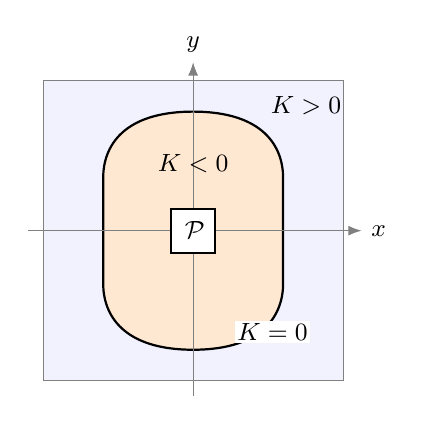
\begin{tikzpicture}[font=\small,>=Latex]
  \begin{scope}[scale=1.12]
    \fill[blue!5] (-1.7,-1.7) rectangle (1.7,1.7);
    \fill[orange!18]
      (0,1.35) .. controls (.80,1.35) and (1.02,.95) .. (1.02,.60)
      -- (1.02,-.60)
      .. controls (1.02,-.95) and (.80,-1.35) .. (0,-1.35)
      .. controls (-.80,-1.35) and (-1.02,-.95) .. (-1.02,-.60)
      -- (-1.02,.60)
      .. controls (-1.02,.95) and (-.80,1.35) .. (0,1.35);
    \draw[thick]
      (0,1.35) .. controls (.80,1.35) and (1.02,.95) .. (1.02,.60)
      -- (1.02,-.60)
      .. controls (1.02,-.95) and (.80,-1.35) .. (0,-1.35)
      .. controls (-.80,-1.35) and (-1.02,-.95) .. (-1.02,-.60)
      -- (-1.02,.60)
      .. controls (-1.02,.95) and (-.80,1.35) .. (0,1.35);
    \draw[gray] (-1.7,-1.7) rectangle (1.7,1.7);
    \draw[->,gray] (-1.87,0)--(1.91,0) node[right,black] {\(x\)};
    \draw[->,gray] (0,-1.87)--(0,1.91) node[above,black] {\(y\)};
    \fill[white] (-.25,-.25) rectangle (.25,.25);
    \draw[thick] (-.25,-.25) rectangle (.25,.25);
    \node at (.02,.01) {\(\mathcal P\)};
    \node at (.0,.76) {\(K<0\)};
    \node at (1.28,1.42) {\(K>0\)};
    \node[fill=white,inner sep=1pt] at (.90,-1.15) {\(K=0\)};
  \end{scope}
\end{tikzpicture}
\caption{The model patch, schematically and not to scale.
The curvature zero set lies outside the perturbation box
\(\mathcal P\). The positive exterior permits estimates on lower and
upper caps whose free artificial edges may cut through the negative
region. The lower-cap integration region is shown in \Cref{fig:cap}.}
\label{fig:geometry}
\end{figure}


\section{Uniform regularity on caps}\label{sec:caps}

The purpose of this section is to turn low-order control of an
admissible height into all-orders control wherever the metric has
all-orders control in a lower or upper cap. The edge facing the
center is artificial: no high-order boundary data will be imposed
there.

Throughout this section we consider families of metrics \(g\in\mathcal U\)
and admissible heights \(z\). Assume fixed uniform bounds
\begin{equation}\label{eq:low-bounds}
\norm g_{C^8(S)}+\norm z_{C^8(S)}\le M,\qquad
g\ge cI,\qquad \abs{H_{yy}}\ge c,\qquad E\ge c,
\end{equation}
where \(M<\infty\) and \(c>0\). Constants in this section may depend
on these bounds, on \(\kappa,h\), and on the derivative order.

Set
\begin{equation}\label{eq:DGa}
D=\pd_x-q\pd_y,\qquad G=\frac E{H_{yy}^2},\qquad a=KG.
\end{equation}
Use flow coordinates \(t,s\) defined by
\begin{equation}\label{eq:flow}
x=t,\qquad y_t(t,s)=-q(t,y(t,s)),\qquad y(0,s)=s.
\end{equation}
They exist on \([-2,2]^2\), have image in the interior of \(S\),
and satisfy
\begin{equation}\label{eq:flow-bounds}
\abs{y(t,s)-s}\le1/50,\qquad D=\pd_t,\qquad
0<c_0\le s_y\le C_0.
\end{equation}
Indeed the first estimate follows from \(\abs q\le1/100\).
Differentiating the flow gives
\[
y_s=\exp\left(-\int_0^t q_y(r,y(r,s))\dd r\right)>0.
\]
The low bounds give uniform bounds for the derivatives of the chart
and its inverse through the orders used below, in particular through
order three. Denote this chart by \(\Phi_z(t,s)=(t,y(t,s))\).

\begin{proposition}[Cap regularity]\label{prop:cap}
Fix \(-1/4<b_*\le0\), and assume \eqref{eq:low-bounds}.
Suppose that, for every compact rectangle
\[
R\Subset(-2,2)\times(-2,b_*),
\]
the ordinary coordinate derivatives of \(g\) of every order have
uniform bounds on \(\Phi_z(R)\).
Then the ordinary coordinate derivatives of \(z\) of every order
also have uniform bounds on \(\Phi_z(R)\).
The corresponding assertion holds for the upper cap
\((-2,2)\times(-b_*,2)\).
\end{proposition}

Here and below a rectangle has sides parallel to the \(t,s\) axes.
Its image may depend on the solution, but all margins in coordinate
labels are chosen independently of the member of the family.
More precisely, if \(R\Subset R'\) are two such rectangles, the
uniform bounds for the chart and its inverse give a fixed radius
of ordinary coordinate balls around points of \(\Phi_z(R)\)
that stay inside \(\Phi_z(R')\). We can therefore apply local
Sobolev estimates with uniform constants in the original coordinates.
No high derivatives of the chart are needed for this step.

\subsection{The differentiated equation}

At the induction step we estimate \(u=\pd_y^lz\) first; the
Darboux equation then recovers derivatives with more \(x\) indices.
We differentiate in the original coordinates before passing to
the flow chart, whose high derivatives are not yet controlled.
Solving the Darboux equation for \(z_{xx}\) gives
\begin{equation}\label{eq:P}
z_{xx}=P(x,y,z_i,z_{xy},z_{yy})
=\Gamma^r_{xx}z_r+\frac{H_{xy}^2+KE}{H_{yy}}.
\end{equation}
The metric and its derivatives are prescribed arguments of \(P\).
In particular,
\begin{equation}\label{eq:P-partials}
P_{z_{xy}}=2q,\qquad P_{z_{yy}}=-q^2-a,\qquad
P_{z_i}=\Gamma^i_{DD}+O(K).
\end{equation}
The notation \(\Gamma^i_{DD}\) contracts the two lower Christoffel
indices against \(D\), without differentiating \(D\).
The last identity follows more explicitly from
\[
P_{z_i}=\Gamma^i_{DD}
+K\left(\frac{E_{z_i}}{H_{yy}}
+\frac{E\Gamma^i_{yy}}{H_{yy}^2}\right).
\]
All coefficients in an \(O(K)\) term in this section are uniformly
bounded under \eqref{eq:low-bounds}.

\begin{lemma}[Curvature drift]\label{lem:drift}
The quantities in \eqref{eq:DGa} satisfy
\begin{equation}\label{eq:drift}
Dq-P_{z_x}q-P_{z_y}=K_yG+O(K).
\end{equation}
\end{lemma}

\begin{proof}
Put \(Y=\pd_y\). The definitions and the Darboux equation give
\[
H(Y,D)=0,\qquad H(D,D)=KE/H_{yy},
\qquad H(D,\pd_x)=KE/H_{yy}.
\]
Thus \(H(D,\cdot)=O(K)\) on bounded coordinate vectors.
The commutation formula for a covariant Hessian gives
\begin{equation}\label{eq:hessian-commutation}
(\nabla_DH)(Y,D)=(\nabla_YH)(D,D)+O(K),
\end{equation}
because in dimension two the curvature tensor is a bounded tensor
multiple of \(K\), and the commutator contracts it against \(dz\).

Differentiate \(H(Y,D)=0\). The term containing \(\nabla_DY\)
is \(O(K)\), and
\(\nabla_DD=\Gamma^i_{DD}\pd_i-(Dq)Y\). Hence the left side
of \eqref{eq:hessian-commutation} equals
\[
H_{yy}(Dq-q\Gamma^x_{DD}-\Gamma^y_{DD})+O(K).
\]
On the right, differentiating \(H(D,D)=KE/H_{yy}\) gives
\(K_yE/H_{yy}+O(K)\); the two connection terms are \(O(K)\).
Division by \(H_{yy}\), followed by \eqref{eq:P-partials},
proves \eqref{eq:drift}.
\end{proof}

\begin{lemma}[High derivative equation]\label{lem:high-equation}
Let \(l\ge8\). Suppose that the ordinary derivatives of \(z\) through
order \(l\) have uniform \(L^2\) bounds on images of compact rectangles
in the lower cap, and that the metric satisfies the hypothesis of
\Cref{prop:cap}. Then \(u=\pd_y^l z\), re-expressed in flow coordinates,
satisfies
\begin{equation}\label{eq:linear-cap}
u_{tt}+Au_{ss}+Bu_t+Cu_s=R_l,
\end{equation}
where \(R_l\) is uniformly bounded in \(L^2\) on smaller compact
rectangles, and
\begin{equation}\label{eq:linear-coefficients}
\begin{gathered}
A=G_1K,\qquad G_1=Gs_y^2,\qquad
B=-P_{z_x}-2lq_y,\\
C=(l+1)A_s+O_l(A).
\end{gathered}
\end{equation}
The function \(G_1\) has positive lower and upper bounds and bounded
first derivatives. The coefficients \(A,A_t,A_s,B,B_s,C\) are
uniformly bounded.
\end{lemma}

\begin{proof}
The inductive \(L^2\) bounds give supremum bounds through order
\(l-2\) on smaller sets by the local two-dimensional Sobolev
inequality on the ordinary coordinate balls described above.

Differentiate \eqref{eq:P} \(l\) times in the original \(y\)
coordinate. In addition to the direct linearization, the terms
containing derivatives of \(z\) of order \(l+1\) are
\[
l\bigl(2q_yu_x-(q^2+a)_yu_y\bigr).
\]
These arise when a second-jet argument receives \(l-1\)
differentiations and the remaining single derivative is placed
elsewhere. The coefficient derivatives are total derivatives,
including the explicit metric dependence of \(P\).

Every remaining differentiated solution factor has order at most
\(l\). A factor of order at least \(l-1\) consumes at least \(l-3\)
of the \(l\) differentiations. There cannot be two such factors,
since \(2(l-3)>l\) for \(l\ge8\). Thus all but at most one factor
use the supremum bounds through order \(l-2\); the remaining factor
uses its \(L^2\) bound. Metric derivatives are bounded by hypothesis,
and inverse powers of \(H_{yy}\) are bounded by
\eqref{eq:low-bounds}. The remainder is consequently bounded in
\(L^2\).

Using
\[
D^2=\pd_x^2-2q\pd_{xy}+q^2\pd_y^2-(Dq)\pd_y
\]
and \(\pd_x=D+q\pd_y\), the differentiated equation becomes
\begin{equation}\label{eq:pre-flow}
\left[
D^2+a\pd_y^2+BD+
\bigl(Dq-P_{z_x}q-P_{z_y}+la_y\bigr)\pd_y
\right]u=R_l.
\end{equation}
Now \(D=\pd_t\), \(\pd_y=s_y\pd_s\), and
\(\pd_y^2=s_y^2\pd_s^2+s_{yy}\pd_s\).
By \Cref{lem:drift}, the transverse coefficient is
\[
C=a s_{yy}+s_y(K_yG+la_y+O(K))
=(l+1)Gs_yK_y+O_l(K).
\]
Since
\[
A_s=Gs_yK_y+K(Gs_y^2)_s,
\]
this is \eqref{eq:linear-coefficients}. The factor \(l+1\) has two
sources: the commutation identity contributes one copy of
\(Gs_yK_y\), and the term \(la_y\) contributes \(l\) copies.
Every other transverse term contains \(K\) times a bounded factor.
All asserted low coefficient
bounds follow from \eqref{eq:low-bounds} and the flow bounds.
\end{proof}

\subsection{A weighted gradient estimate}

The differentiated equation reduces the cap induction to a gain
of one derivative. Its principal part changes type, so an elliptic
estimate alone is insufficient. We combine a directed multiplier
near and inside the negative region with a weighted elliptic
estimate on its complement.

\begin{lemma}[The free cap edge]\label{lem:gradient}
Retain the model geometry and flow coordinates fixed above.
Let \(l\ge8\), and let the coefficients satisfy
\eqref{eq:linear-coefficients} with the uniform bounds in
\Cref{lem:high-equation}. For every
\(R_0\Subset(-2,2)\times(-2,b_*)\), there is a larger compact
rectangle \(R_1\) in that cap and a constant \(C_{R_0,l}\) such that
every smooth solution of
\[
u_{tt}+Au_{ss}+Bu_t+Cu_s=f
\]
on a neighborhood of \(R_1\) satisfies
\begin{equation}\label{eq:gradient-bound}
\norm{(u_t,u_s)}_{L^2(R_0)}
\le C_{R_0,l}\bigl(\norm u_{L^2(R_1)}+\norm f_{L^2(R_1)}\bigr).
\end{equation}
The constants are uniform over the families under consideration.
\end{lemma}

\begin{proof}
Choose \(b<b_*\) above the upper edge of \(R_0\).
Integrations will take place below \(s=b\), with their other three
edges sufficiently far out that cutoff derivatives lie in
\[
3/2<\abs t<2
\quad\text{or}\quad -2<s<-3/2.
\]
Both regions have uniformly positive curvature. At the lateral
edges, \(t^2-h(y)\ge t^2-1>0\). At the lower edge,
\eqref{eq:flow-bounds} gives \(y<-1\), so \(h(y)<0\).
There is room for nested cutoffs there and for a compact rectangle
\(R_1\) containing every integration set, including its upper edge.

Set \(d=b-s\) and \(p=8\). We choose the directed weight to vanish
like \(d^p\) at the artificial edge; it remains positive on \(R_0\).
Differentiating such a weight costs a factor \(d^{-1}\), so the
two estimates will meet at \(K=c_1d\), for a small constant
\(c_1>0\) chosen below. The directed multiplier controls
\(K\le c_1d\), where its positive-curvature error is
\(O(K/d)\). On \(K\ge c_1d\), an elliptic estimate controls
the stronger weight \(d^{p-1}\), which pays for the weight and
cutoff derivatives. \Cref{fig:cap} shows the integration geometry.

\begin{figure}[H]
\centering
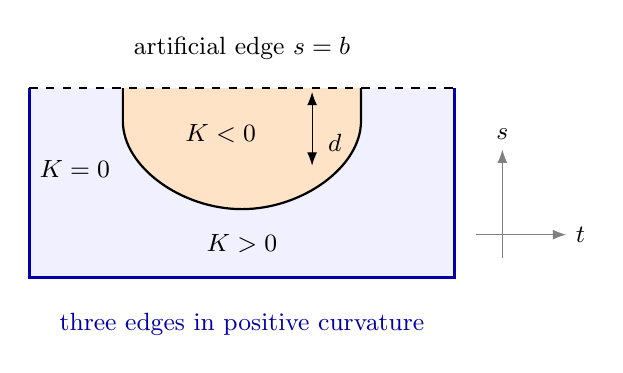
\begin{tikzpicture}[font=\small,>=Latex,xscale=1.35,yscale=1.2]
  \fill[blue!6] (-2,-2) rectangle (2,0);
  \fill[orange!22]
    (-1.12,0)--(-1.12,-.35)
    .. controls (-1.12,-.83) and (-.57,-1.28) .. (0,-1.28)
    .. controls (.57,-1.28) and (1.12,-.83) .. (1.12,-.35)
    --(1.12,0)--cycle;
  \draw[thick]
    (-1.12,0)--(-1.12,-.35)
    .. controls (-1.12,-.83) and (-.57,-1.28) .. (0,-1.28)
    .. controls (.57,-1.28) and (1.12,-.83) .. (1.12,-.35)
    --(1.12,0);
  \draw[very thick,blue!65!black] (-2,0)--(-2,-2)--(2,-2)--(2,0);
  \draw[thick,dashed] (-2,0)--(2,0);
  \node[above=7pt] at (0,0) {artificial edge \(s=b\)};
  \node at (-.2,-.48) {\(K<0\)};
  \node at (0,-1.65) {\(K>0\)};
  \node[anchor=east] at (-1.15,-.85) {\(K=0\)};
  \draw[<->] (.66,-.04)--(.66,-.82);
  \node[anchor=west] at (.72,-.58) {\(d\)};
  \draw[->,gray] (2.45,-1.8)--(2.45,-.65) node[above,black] {\(s\)};
  \draw[->,gray] (2.2,-1.55)--(3.05,-1.55) node[right,black] {\(t\)};
  \node[text=blue!65!black] at (0,-2.5) {three edges in positive curvature};
\end{tikzpicture}
\caption{A lower-cap integration region in flow coordinates, schematically
and not to scale. The lateral and bottom edges are chosen in positive
curvature. The artificial edge \(s=b\) may cross the negative region;
no high-order data are prescribed there. The distance \(d=b-s\)
enters the vanishing weight. The actual curvature zero set depends on
the solution through the flow coordinates; only its position relative
to the three elliptic edges and the artificial edge is illustrated.}
\label{fig:cap}
\end{figure}


\smallskip
\noindent\emph{The directed multiplier.}
The transverse multiplier uses the favorable curvature drift.
We add a small \(t\)-directed part to obtain positivity at those
zeros of curvature where \(K_y=0\): there the \(x^2\) term in
the model curvature must supply the estimate.
Put
\begin{equation}\label{eq:weights}
\begin{gathered}
I(t,s)=\int_0^tB(r,s)\dd r,\\
W=d^p e^{-\lambda s+I(t,s)},\qquad
m=-W,\qquad n=\epsilon tW,\qquad H_0=\lambda+p/d .
\end{gathered}
\end{equation}
Here \(\epsilon>0\) will be small and \(\lambda>0\) large.
The factor \(e^I\) gives \(m_t=Bm\), canceling the corresponding
mixed term in the identity below. Also
\(m_s/W=H_0-I_s\), with \(I_s\) uniformly bounded.

Testing against \(mu_s+nu_t\) and integrating by parts gives
the interior quadratic form
\begin{equation}\label{eq:quadratic}
T u_t^2+S_0u_s^2+Ju_tu_s,
\qquad
\begin{cases}
T=(m_s-n_t)/2+Bn,\\
S_0=-(Am)_s/2+(An)_t/2+Cm,\\
J=-m_t+Bm-(An)_s+Cn.
\end{cases}
\end{equation}
The symbol \(S_0\) denotes this coefficient, not the model square.
Substituting \eqref{eq:weights} gives, for large \(\lambda\),
\begin{equation}\label{eq:quadratic-bounds}
\begin{aligned}
T/W&\ge H_0/4,\\
S_0/W&=-(l+1/2)A_s+\epsilon tA_t/2-H_0A/2+O_l(A),\\
\abs J/W&\le C_l\epsilon(1+H_0\abs A).
\end{aligned}
\end{equation}

\smallskip
\noindent\emph{Positivity near and inside the negative region.}
There are choices of these constants and \(c_1,c_2>0\) such that
\begin{equation}\label{eq:coercive}
T u_t^2+S_0u_s^2+Ju_tu_s
\ge c_2W(u_t^2+u_s^2)
\qquad\text{where }K\le c_1d.
\end{equation}
We verify the choices in detail.

For \(\abs K\) sufficiently small, \eqref{eq:negative-box}
excludes \(\mathcal P\), so the prescribed curvature formula applies.
In the lower cap \(y\le1/50\). The plateau and monotonicity in
\eqref{eq:h} imply \(K_y\le0\) there. Also
\begin{equation}\label{eq:A-derivatives}
A_s=G_1K_y/s_y+O(A),\qquad
A_t=G_1(2\kappa t-qK_y)+O(A).
\end{equation}
Thus the first two terms in the second line of
\eqref{eq:quadratic-bounds}, up to \(O_l(A)\), equal
\[
G_1\left[
-\left(\frac{l+1/2}{s_y}+\frac{\epsilon tq}{2}\right)K_y
+\epsilon\kappa t^2
\right].
\]
For small fixed \(\epsilon>0\) this is bounded below by a positive
constant times \(-K_y+\epsilon t^2\). To make its uniform
positivity independent of the flow chart, consider the fixed
physical zero set
\[
\mathcal Z=\{(x,y)\in[-2,2]\times[-101/50,1/50]:x^2=h(y)\}.
\]
It is compact and contains every curvature zero in the lower cap.
If \(x=0\) on \(\mathcal Z\), then \(y=-1\), where \(K_y<0\);
at every other point \(x^2>0\). Thus
\(-K_y+\epsilon x^2\) has a positive minimum on \(\mathcal Z\).
The uniform bounds for \(G_1,s_y,q\) transfer this minimum to
the geometric contribution on a common neighborhood of \(K=0\).

The cross-term loss after absorbing part of \(T u_t^2\) is bounded by
\begin{equation}\label{eq:cross-loss}
\frac{J^2}{TW}
\le C_l'\epsilon^2\left(H_0^{-1}+H_0A^2\right).
\end{equation}
On \(K\le0\), the term \(-H_0A/2=H_0\abs A/2\) is favorable.
Since \(\abs A\) is bounded, choose \(\epsilon\) small enough
to absorb the second term of \eqref{eq:cross-loss} into a small
fraction of \(H_0\abs A\). Increase \(\lambda\) to absorb
the \(O_l(A)\) terms and the \(H_0^{-1}\) loss.
Away from a neighborhood of the zero set on the negative side,
the same increase of \(\lambda\) makes \(H_0\abs A\) dominate
all bounded adverse terms.

Fix these \(\epsilon,\lambda\). On \(0<K\le c_1d\), since \(d\)
is bounded above,
\[
H_0A\le Cc_1(\lambda d_{\max}+p).
\]
Choose \(c_1\) so small that this region lies in the preceding
neighborhood of the zero set, and that the adverse \(H_0A\)
term and remaining errors use only a fraction of its positive
lower bound. This proves \eqref{eq:coercive}. The order of
choices is \(\epsilon\), then \(\lambda\), then \(c_1\).

\smallskip
\noindent\emph{The auxiliary elliptic estimate.}
On the remaining region we claim
\begin{equation}\label{eq:aux-elliptic}
\iint_{\{K\ge c_1d\}} d^{p-1}(u_t^2+u_s^2)\dd t\dd s
\le C\bigl(\norm u_{L^2(R_1)}^2+\norm f_{L^2(R_1)}^2\bigr),
\end{equation}
on any of the supports needed for the directed multiplier.
To prove it, choose a cutoff \(\chi\) farther out at the three
elliptic edges, equal to one on those supports. Let \(\phi\) be
a smooth cutoff equal to zero on \((-\infty,c_1/2]\) and one
on \([c_1,\infty)\), and test the equation against \(-vu\), where
\[
v=d^{p-2}\chi^2\phi(K/d)^2.
\]
On \(v>0\), \(A\ge c'd\). In the transition region of \(\phi\),
\(K=O(d)\), and hence derivatives of \(K/d\) are \(O(d^{-1})\).
It follows that
\[
\abs{v_t}+\abs{v_s}
\le C\sqrt v\,d^{(p-2)/2}(1+d^{-1}).
\]
The squared cutoffs make this inequality valid also at their zeros.

Integration by parts produces the positive term
\(\iint v(u_t^2+Au_s^2)\) and the error
\[
\iint u\bigl[(v_t-vB)u_t+((Av)_s-vC)u_s\bigr].
\]
On \(v>0\), the coefficient bounds and \(A\ge c'd\) give
\[
\frac{(v_t-vB)^2}{v}
+\frac{((Av)_s-vC)^2}{Av}
\le C(1+d^{p-5}).
\]
Young's inequality absorbs half of the positive term; the remaining
cost is at most \(C\iint(1+d^{p-5})u^2\).
Since \(p=8\), this is bounded by \(C\norm u_2^2\).
The source term is at most \(C\norm f_2\norm u_2\).
We conclude that
\[
\iint v(u_t^2+Au_s^2)
\le C(\norm u_2^2+\norm f_2^2).
\]
Where \(\chi=\phi=1\), \(v=d^{p-2}\gtrsim d^{p-1}\)
and \(vA\gtrsim d^{p-1}\), proving \eqref{eq:aux-elliptic}.
This estimate permits ellipticity to degenerate linearly as
\(s\) approaches \(b\).

\smallskip
\noindent\emph{Combining the estimates.}
Multiply \(m,n\) by one nonnegative cutoff toward the other three
edges, equal to one on \(R_0\) and on the nonelliptic portion of
the integration region. Its derivative terms lie in fixed positive
curvature; decreasing \(c_1\), if needed, puts those supports
in the region controlled by \eqref{eq:aux-elliptic}.
The coefficients in \eqref{eq:quadratic} and the cutoff errors
are \(O(d^{p-1})\), since \(W\asymp d^p\) and \(H_0=O(1+d^{-1})\).
Thus \eqref{eq:aux-elliptic} controls all adverse terms outside
\eqref{eq:coercive}.

On the coercive region the source \(f(mu_s+nu_t)\) is absorbed by
Young's inequality, at a cost \(C\norm f_2^2\). On the complementary
region use \eqref{eq:aux-elliptic} and
\(W^2/d^{p-1}=O(d^{p+1})\) to obtain the same bound together
with \(C\norm u_2^2\). Combining the coercive part with the
elliptic estimate on its complement, we obtain
\[
\iint_{R_0}W(u_t^2+u_s^2)
\le C(\norm u_{L^2(R_1)}^2+\norm f_{L^2(R_1)}^2).
\]
The weight is bounded below on \(R_0\), so this proves
\eqref{eq:gradient-bound}.

All integrations at the artificial edge can first be made below
\(s=b-\eta\) and then continued to \(\eta=0\).
For each individual smooth solution, the boundary terms vanish
because \(W\) and \(v\) vanish to positive order. The edge \(b\)
is strictly inside the smooth domain. No uniform bound on its
high derivatives is needed to obtain these identities; the uniform
estimates involve only the interior \(L^2\) norms just displayed.
\end{proof}

\subsection{Completion of the cap induction}

\begin{proof}[Proof of \Cref{prop:cap}]
We prove uniform \(L^2\) bounds for ordinary derivatives of \(z\)
through order \(l\), on images of all compact rectangles in the
cap. The case \(l=8\) follows from \eqref{eq:low-bounds}.
Assume the assertion at some \(l\ge8\). Apply
\Cref{lem:high-equation,lem:gradient} with \(f=R_l\).
The required bounds for \(u,R_l\) on the larger compact rectangle
are supplied by the induction hypothesis. Measures in the two
coordinate systems are uniformly comparable.

The resulting gradient bound controls
\[
\pd_y^{l+1}z=s_yu_s,\qquad
\pd_x\pd_y^lz=u_t+q s_yu_s.
\]
To recover \(\pd_x^k\pd_y^{l+1-k}z\) for \(k\ge2\), apply
\(\pd_x^{k-2}\pd_y^{l+1-k}\) to \eqref{eq:P}.
The two top terms on the right are
\[
P_{z_{xy}}\pd_x^{k-1}\pd_y^{l+2-k}z
\quad\text{and}\quad
P_{z_{yy}}\pd_x^{k-2}\pd_y^{l+3-k}z.
\]
They have fewer \(x\) indices. All remaining solution factors
have order at most \(l\) and obey the same Sobolev product bounds
as in \Cref{lem:high-equation}. Increasing \(k\) therefore gives
every derivative of order \(l+1\).

This closes the induction. For each fixed derivative order, local
Sobolev estimates on slightly larger compact rectangles convert
the \(L^2\) bounds into the asserted supremum bounds. The final
rectangle is arbitrary and fixed; only the constants and intermediate
margins depend on the derivative order.
Reflection \(y\mapsto-y\), using the evenness of \(h\), proves
the upper-cap assertion.
\end{proof}

\section{The oscillatory pulse and the patch obstruction}\label{sec:pulse}

We now prove \Cref{prop:patch} by a category argument. Assuming
density of a class of metrics admitting uniformly bounded heights,
we perturb a fixed metric inside a thin strip. Cap regularity and hyperbolic propagation give
smooth tangential data at both strip edges for every corresponding
height. A Taylor comparison for the fixed metric isolates the change
in the transverse derivative caused by the perturbation. Its
oscillatory moment is incompatible with smooth data at both edges.

\subsection{A bounded solution class}

The vector space of smooth symmetric tensors supported in
\(\mathcal P\) is a closed subspace of a smooth-function Fréchet
space. Its open subset \(\mathcal U\) is therefore a Baire space.
For \(M\in\N\), consider metrics admitting an admissible height with
\begin{equation}\label{eq:class-bounds}
\norm z_{C^8(S)}\le M,\qquad
M^{-1}\le\abs{H_{yy}}\le M,\qquad E\ge M^{-1}.
\end{equation}
Put
\begin{equation}\label{eq:speed-constants}
v_*=\sqrt{\kappa/2}\,M^{-3/2},\qquad
L=100(1+v_*^{-1}).
\end{equation}
For each rational \(q_0\), let \(\mathcal A_{M,q_0}\) be the
subclass in which such a height also satisfies
\begin{equation}\label{eq:q-class}
\abs{q(0,0)-q_0}<\frac1{100L}.
\end{equation}
These countably many classes cover every metric with an admissible
height. Indeed smoothness and the strict inequalities on the compact
square supply some \(M\), after which rational approximation supplies
\(q_0\). We will show that each class is nowhere dense.

Suppose, to the contrary, that the closure of one class contains a
nonempty open set \(\mathcal O\subset\mathcal U\). Fix
\(g_*\in\mathcal O\). All test metrics below lie in \(\mathcal O\)
and converge to \(g_*\) in \(C^8\). Metrics from the class can
be chosen arbitrarily close to each test metric in the smooth
topology. We may consequently use uniform low bounds for the metric,
its inverse, and the first derivatives of \(q\).
Since \(\abs q\le1/100\), a nonempty class satisfies
\(\abs{q_0}<1/20\).

Introduce linear coordinates
\begin{equation}\label{eq:shear}
\xi=x,\qquad \theta=y+q_0x.
\end{equation}
On a sufficiently small fixed neighborhood of the center, the
preceding low bounds imply
\begin{equation}\label{eq:central-bounds}
\abs{q-q_0}\le\frac1{10L},
\qquad \sqrt{-a}\ge v_*.
\end{equation}
The second inequality follows from \eqref{eq:negative-box}
and \eqref{eq:class-bounds}. In these coordinates,
\begin{equation}\label{eq:sheared-hessian}
\begin{gathered}
H_{\theta\theta}=H_{yy},\qquad
H_{\xi\theta}=(q-q_0)H_{yy},\\
H_{\xi\xi}=d_0H_{yy},\qquad d_0=(q-q_0)^2+a.
\end{gathered}
\end{equation}
Because \((10L)^{-1}\le v_*/1000\), \(d_0<0\) is separated
from zero. Solving the height equation in the other direction gives
\begin{equation}\label{eq:Q}
z_{\theta\theta}
=Q_g(\xi,\theta,z_i,z_{\xi\xi},z_{\theta\xi})
=\Gamma^i_{\theta\theta}z_i+
\frac{H_{\theta\xi}^2+(K\det g)(1-\abs{dz}_g^2)}
     {H_{\xi\xi}}.
\end{equation}
Its second-jet partial derivatives, at a solution, are
\begin{equation}\label{eq:hyperbolic-coefficients}
P_1=Q_{z_{\theta\xi}}=\frac{2(q-q_0)}{d_0},
\qquad S_1=Q_{z_{\xi\xi}}=-\frac1{d_0}>0.
\end{equation}
They have bounded first derivatives; \(S_1\) has a positive lower
bound. The following convenient speed bound follows from
\eqref{eq:central-bounds}:
\begin{equation}\label{eq:speed-bound}
\abs{P_1}+\sqrt{S_1}\le4/v_*<L/4.
\end{equation}

Choose \(r>0\) small enough that the slab
\begin{equation}\label{eq:slab}
-r\le\theta\le r,\qquad \abs\xi\le Lr
\end{equation}
and fixed margins lie in the preceding neighborhood and inside
\(\mathcal P\). We also require \(r<1/2\).
Along a flow line from \eqref{eq:flow},
\(D\theta=q_0-q\), whereas \(\theta=s\) when \(t=0\).
The global bound \(\abs q\le1/100\) keeps these flow segments
in that neighborhood after a further shrinking of \(r\). Thus throughout
the slab
\begin{equation}\label{eq:s-theta}
\abs{s-\theta}\le r/4.
\end{equation}
In fact the bound \(r/10\) follows from its \(t\)-length at most \(Lr\).

\subsection{The test metrics and smooth data at the pulse edges}

Choose a nonzero real \(\chi_0\in C_c^\infty((-Lr/8,Lr/8))\) and
a nonnegative \(\phi_0\in C_c^\infty((-1,1))\) with
\(\int\phi_0>0\). For small fixed \(\delta>0\) and integers
\(\tau\to\infty\), the test metrics are
\begin{equation}\label{eq:pulse}
\widetilde g_\tau
=g_*+\tau^{-N}\chi_0(\xi)\phi_0(\tau\theta/\delta)
                 \cos(\tau\xi)\dd\theta^2.
\end{equation}
Choose the fixed integer \(N>10\) larger than every derivative order
in one basic neighborhood of \(g_*\) contained in \(\mathcal O\).
For each fixed \(\delta\), the test metrics then belong to
\(\mathcal O\) for all sufficiently large \(\tau\). Only finitely
many seminorms are involved in this assertion.

By the closure assumption choose \(g_\tau\in\mathcal A_{M,q_0}\)
such that
\begin{equation}\label{eq:approximation}
\norm{g_\tau-\widetilde g_\tau}_{C^\tau(S)}
\le\tau^{-\tau},
\end{equation}
and choose a corresponding height \(z_\tau\) with
\eqref{eq:class-bounds} and \eqref{eq:q-class}.
We suppress its subscript when deriving estimates.
All comparisons using finitely many low derivatives hold uniformly
for large \(\tau\). Their limiting constants can be chosen independently
of the fixed small \(\delta\), since \(N>10\).

Away from the pulse rectangle
\[
\abs\theta\le\delta/\tau,\qquad \abs\xi\le Lr/8,
\]
the metrics have uniform bounds at every fixed derivative order.
By \eqref{eq:s-theta}, every point of that rectangle has
\(\abs s<r/2\) for large \(\tau\), in every solution's flow chart.
Consequently the image of every compact rectangle in
\((-2,2)\times(-2,-r/2)\), or in
\((-2,2)\times(r/2,2)\), misses the pulse support. On all such
images, \(g_\tau\) differs from the fixed metric \(g_*\) only
by the approximation error \eqref{eq:approximation}. This verifies
the metric hypothesis of \Cref{prop:cap} throughout both caps,
with \(b_*=-r/2\). The proposition gives bounds for every
derivative of \(z\) on the two cuts
\begin{equation}\label{eq:cap-cuts}
\theta=\pm r,\qquad \abs\xi\le Lr.
\end{equation}
These cuts lie in compact subsets of the respective flow-coordinate
caps, uniformly over the solutions.
\Cref{fig:pulse} shows the cuts and the pulse inside the
negative-curvature slab.

\begin{figure}[H]
\centering
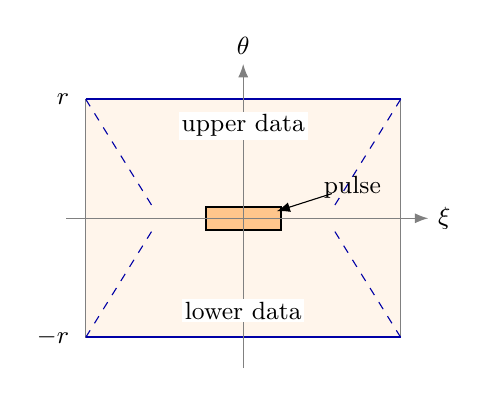
\begin{tikzpicture}[font=\small,>=Latex,xscale=1.25,yscale=1.12]
  \fill[orange!8] (-1.6,-1.35) rectangle (1.6,1.35);
  \draw[gray] (-1.6,-1.35) rectangle (1.6,1.35);
  \draw[thick,blue!65!black] (-1.6,-1.35)--(1.6,-1.35);
  \draw[thick,blue!65!black] (-1.6,1.35)--(1.6,1.35);
  \draw[blue!65!black,dashed] (-1.6,-1.35)--(-.92,-.13);
  \draw[blue!65!black,dashed] (1.6,-1.35)--(.92,-.13);
  \draw[blue!65!black,dashed] (-1.6,1.35)--(-.92,.13);
  \draw[blue!65!black,dashed] (1.6,1.35)--(.92,.13);
  \fill[orange!45] (-.38,-.13) rectangle (.38,.13);
  \draw[thick] (-.38,-.13) rectangle (.38,.13);
  \draw[->,gray] (-1.8,0)--(1.88,0) node[right,black] {\(\xi\)};
  \draw[->,gray] (0,-1.70)--(0,1.75) node[above,black] {\(\theta\)};
  \node[anchor=east] at (-1.67,-1.35) {\(-r\)};
  \node[anchor=east] at (-1.67,1.35) {\(r\)};
  \node[fill=white,inner sep=1pt] at (0,1.05) {upper data};
  \node[fill=white,inner sep=1pt] at (0,-1.05) {lower data};
  \draw[->] (.9,.28)--(.34,.08);
  \node[anchor=west] at (.72,.35) {pulse};
\end{tikzpicture}
\caption{The hyperbolic slab, schematically and not to scale.
Cap regularity gives smooth data on the two cuts \(\theta=\pm r\).
The dashed lines indicate the shrinking spatial intervals used to
propagate those data toward both pulse edges. The pulse is supported
in \(\abs\theta<\delta/\tau\) and oscillates in \(\xi\).
The entire slab lies in negative curvature.}
\label{fig:pulse}
\end{figure}


\begin{lemma}[Propagation to the pulse]\label{lem:propagation}
At \(\theta=\pm\delta/\tau\), on \(\abs\xi\le Lr/2\),
the functions \(z,z_\theta\) have uniform bounds for every
tangential derivative.
\end{lemma}

\begin{proof}
We record the energy argument, which will also be used on the pulse.
If \(v\) satisfies
\[
v_{\theta\theta}-P_1v_{\theta\xi}-S_1v_{\xi\xi}
=b^\theta v_\theta+b^\xi v_\xi+R,
\]
with the above coefficient bounds and bounded \(b^i\), use the energy
density and flux
\[
e=\frac{v_\theta^2+S_1v_\xi^2}{2},
\qquad
j=\frac{P_1v_\theta^2}{2}+S_1v_\xi v_\theta.
\]
One has
\(\abs j\le(\abs{P_1}+\sqrt{S_1})e\).
Integrate on intervals whose endpoints move inward at speed \(L/4\).
Multiplication by \(v_\theta\) and integration by parts, with the
nonpositive boundary loss discarded, gives
\begin{equation}\label{eq:energy}
\mathcal E'(\theta)
\le C\mathcal E(\theta)
+\sqrt{2\mathcal E(\theta)}\,\norm R_{L^2},
\qquad \mathcal E(\theta)=\int e\dd\xi.
\end{equation}
Thus \(\sqrt{\mathcal E}\) is controlled by its initial value and
the time integral of \(\norm R_2\), with a Gronwall factor.
One can justify division at zero energy by first using
\(\sqrt{\mathcal E+\eta}\) and then letting \(\eta\downarrow0\).

Apply this estimate to \(v=\pd_\xi^jz\), \(j\ge8\), obtained by
differentiating \eqref{eq:Q}. The top second-jet terms give
the principal coefficients in \eqref{eq:hyperbolic-coefficients}.
If a second-jet argument receives \(j-1\) differentiations,
it gives \(v_\xi\) or \(v_\theta\); put these terms, together
with the direct first-jet linearization, into \(b^i\pd_iv\).
Their coefficients use only bounded low derivatives.
Put \(V=(z_\xi,z_\theta)\). Every remaining solution factor is
a spatial derivative of \(V\) of order at most \(j-1\),
already controlled by the induction. A factor of order \(j-1\)
requires at least \(j-2\) of the differentiations, since a
second-jet argument is already one spatial derivative of \(V\).
There cannot be two such factors, because \(2(j-2)>j\).
Bound that factor in \(L^2\), if it occurs. All other factors
have order at most \(j-2\), so the one-dimensional Sobolev
inequality and the available \(H^{j-1}\) bound for \(V\)
control them in supremum norm. This gives the \(L^2\) bound
for the remainder in \eqref{eq:energy}.
The same moving interval is used at every derivative order;
its length has a fixed positive lower bound, so the one-dimensional
Sobolev constants are uniform.

The initial first-jet bounds through spatial order seven follow
from the \(C^8\) class bound. For each larger order, the initial
energy on the cut \(\theta=-r\) is bounded by the cap estimate.
The metric derivatives are bounded on
\(-r\le\theta\le-\delta/\tau\), so \eqref{eq:energy}
closes the spatial induction there. The intervals start as
\([-Lr,Lr]\) and lose at most \(Lr/4\) at each end, leaving
room for Sobolev estimates on \(\abs\xi\le Lr/2\).
Reverse time and start at \(\theta=r\) to obtain the same bounds
at the upper pulse edge.
\end{proof}

\subsection{A comparison across the thin strip}

On \(\abs\xi\le Lr/2\), construct a smooth comparison \(z^0\)
on \(-\delta/\tau\le\theta\le\delta/\tau\) with the same data
\((z,z_\theta)\) at \(\theta=-\delta/\tau\), satisfying
\eqref{eq:Q} for the fixed metric \(g_*\) up to \(O(\tau^{-N})\).
For this purpose take the time Taylor polynomial of degree \(N+1\)
at the initial edge. Recursively determine its higher coefficients
from \eqref{eq:Q}, using \(g_*\). At step \(k\), for
\(0\le k\le N-1\), differentiating the right side \(k\) times
determines the time derivative of order \(k+2\) from those
through order \(k+1\) and their spatial derivatives. This is
possible because \(Q_g\) contains no second time derivative.
The denominator at the initial
data stays separated from zero by metric closeness and
\eqref{eq:sheared-hessian}. The coefficients and each fixed spatial
derivative are uniformly bounded by \Cref{lem:propagation}.
The denominator remains nonzero on the short strip. The recurrence
makes the residual and its first \(N-1\) time derivatives vanish
at the initial edge. Taylor's formula on a strip of length
\(2\delta/\tau\) gives the claimed \(O(\tau^{-N})\) bound
for fixed \(\delta\). In particular, \(z^0_\theta\) at the final
edge has bounds for all fixed spatial derivatives.

Put \(w=z-z^0\). Move \(Q_{g_*}(z)-Q_{g_*}(z^0)\) to the
linearized side, using mean partial derivatives along the segments
between their argument vectors
\((z_i,z_{\xi\xi},z_{\theta\xi})\). This yields
\begin{equation}\label{eq:w-equation}
w_{\theta\theta}-P_2w_{\theta\xi}-S_2w_{\xi\xi}
+\beta^i\pd_iw
=Q_{g_\tau}(z)-Q_{g_*}(z)+O(\tau^{-N}),
\end{equation}
with zero Cauchy data at the lower edge.
Here \(S_2>0\) has a uniform lower bound; the coefficients
are bounded and \(P_2,S_2\) have bounded first derivatives.
To see the positivity, the \(C^8\) bound keeps the actual argument
vector close throughout the strip to its initial value. The same is
true of the polynomial, by its coefficient bounds. The argument
vectors agree at the initial edge, because the Cauchy data agree.
At this common value, \(Q_{g_*,z_{\xi\xi}}>0\) by metric closeness and
\eqref{eq:hyperbolic-coefficients}. Continuity keeps it positive
on all the intervening segments, on which the denominator also
remains separated from zero. It is not necessary that those
segments consist of solutions.

A fixed speed bound larger than the one in \eqref{eq:speed-bound}
therefore applies to \eqref{eq:w-equation}. The limiting bounds
for the zeroth-order coefficient values and the positive lower
bound for \(S_2\) are independent of the fixed small \(\delta\).

\subsection{The curvature forcing and its moment}

In the linear coordinates \(\xi,\theta\), the curvature tensor formula
gives
\begin{equation}\label{eq:curvature-density}
K\det g
=\pd_{\xi\theta}g_{\xi\theta}
-\frac{\pd_\xi^2g_{\theta\theta}+\pd_\theta^2g_{\xi\xi}}2
+\mathcal L(g,\pd g),
\end{equation}
where \(\mathcal L\) is smooth for positive metric matrices.
Since \eqref{eq:pulse} changes only \(g_{\theta\theta}\),
its principal contribution is \(-\tfrac12\pd_\xi^2\)
of the scalar pulse. Consequently the right side of
\eqref{eq:w-equation} equals
\begin{equation}\label{eq:forcing}
\tau^{2-N}D_\tau\chi_0(\xi)\phi_0(\tau\theta/\delta)
                   \cos(\tau\xi)+o(\tau^{2-N}),
\qquad
D_\tau=\frac{1-\abs{dz}_{g_*}^2}{2H_{\xi\xi}(g_*,z)}.
\end{equation}
The error is uniform in space and time as \(\tau\to\infty\)
for each fixed \(\delta\). Metric changes involving at most one
derivative are \(O_\delta(\tau^{1-N})\); the approximation
\eqref{eq:approximation} and the Taylor residual are smaller.

There are constants \(c_D,C_D>0\), independent of fixed small
\(\delta\), such that for all large \(\tau\)
\[
c_D\le\abs{D_\tau}\le C_D,
\]
and \(D_\tau\) has one sign throughout the strip used.
Indeed the numerator is bounded below by the \(E\) bound,
uniform metric bounds, and metric closeness. The denominator
has the sign opposite to \(H_{yy}\), by \(d_0<0\), and stays
nonzero when \(g_\tau\) is replaced by \(g_*\).
The sign of \(H_{yy}\) is constant on the connected square.
Upper and lower bounds follow from the same low estimates.

Apply the zero-data estimate \eqref{eq:energy} to
\eqref{eq:w-equation}, shrinking intervals from
\([-Lr/2,Lr/2]\) at a fixed sufficiently large speed.
They contain \(\supp\chi_0\) throughout the strip for large
\(\tau\). Its source has \(L^2\) size \(O(\tau^{2-N})\),
so
\begin{equation}\label{eq:short-energy}
\norm{\pd w}_{L^2}\le(C_2+o(1))\delta\tau^{1-N}
\end{equation}
uniformly in strip time.
Here \(C_2\) can be chosen independently of small fixed
\(\delta\): the strip length is \(2\delta/\tau\), and every
Gronwall factor tends to one for fixed \(\delta\).
Finite coefficient derivative bounds depending on that \(\delta\)
are therefore harmless.

Integrate \eqref{eq:w-equation} against
\(\psi_\tau(\xi)=\chi_0(\xi)\cos(\tau\xi)\) over space and strip time.
The \(w_{\theta\theta}\) term is
\[
\int\psi_\tau(\xi)w_\theta(\xi,\delta/\tau)\dd\xi,
\]
because the initial data vanish. Both \(z_\theta\) and
\(z^0_\theta\) at the final edge have uniform spatial bounds of
every fixed order. Repeated integration by parts therefore makes
this term \(o(\tau^{1-N})\).

For each other second-order term, integrate one spatial derivative
by parts. The derivative of \(\psi_\tau\) costs \(O(\tau)\).
By \eqref{eq:short-energy} and the strip length, the total
absolute cost is at most
\begin{equation}\label{eq:moment-error}
(C_3+o(1))\delta^2\tau^{1-N}.
\end{equation}
The constant \(C_3\) is independent of small fixed \(\delta\);
terms with a derivative on a coefficient and the first-order terms
have an additional factor \(\tau^{-1}\) for fixed \(\delta\).
The spatial test is compactly supported, so there is no spatial
boundary contribution.

In contrast, \eqref{eq:forcing} paired with \(\psi_\tau\)
has absolute integral at least
\begin{equation}\label{eq:moment-lower}
(c_3+o(1))\delta\tau^{1-N},
\qquad c_3>0,
\end{equation}
with \(c_3\) independent of small fixed \(\delta\).
This follows from the constant sign and lower bound of \(D_\tau\),
the nonnegativity and positive integral of \(\phi_0\), and
\[
\int\chi_0(\xi)^2\cos^2(\tau\xi)\dd\xi
\longrightarrow \frac12\int\chi_0(\xi)^2\dd\xi>0.
\]
No convergence of \(D_\tau\) is needed.

Choose \(\delta>0\) so small that \(C_3\delta<c_3/2\),
and then let \(\tau\to\infty\). Equations
\eqref{eq:moment-error} and \eqref{eq:moment-lower} contradict
\eqref{eq:w-equation}.
The order of choices is summarized in \Cref{tab:pulse-choices}.
In particular, no convergence in every smooth seminorm was required
of the test metrics, and no convergence or common sign across
different \(\tau\) was required of \(D_\tau\).

\begin{table}[H]
\centering
\small
\renewcommand{\arraystretch}{1.18}
\begin{tabular}{@{}p{.15\textwidth}p{.36\textwidth}p{.43\textwidth}@{}}
\hline
Stage & Quantities fixed & Dependence permitted\\
\hline
First & Class, neighborhood, \(g_*\), slab, cutoffs, \(N\)
& Fixes leading constants \(C_2,C_3,c_3\), independent of
sufficiently small fixed \(\delta\).\\
Second & \(\delta>0\), with \(C_3\delta<c_3/2\)
& Subsidiary derivative bounds may depend on this fixed \(\delta\).\\
Last & Integers \(\tau\to\infty\)
& Thresholds and little-oh errors may depend on \(\delta\);
the leading constants do not.\\
\hline
\end{tabular}
\caption{Parameter order in the pulse contradiction. Every derivative
order has its own bound; no single bound for all orders is asserted.}
\label{tab:pulse-choices}
\end{table}

We have proved that every \(\mathcal A_{M,q_0}\) is nowhere dense.
Their countable union contains every metric admitting an admissible
height. Baire's theorem now proves \Cref{prop:patch}.

\section{Assembly of a smooth metric germ}\label{sec:assembly}

We now turn the whole-patch obstruction into one metric germ.
There are two levels of accumulation: obstructed patches approach
every boundary point of each negative disk, and the disks approach
the origin. Summable bounds in each derivative order will preserve
smoothness at both levels.
We first recall the elementary prescribed-curvature construction
used in \cite[p.~453]{Khuri2009}.

\begin{lemma}[Prescribing small curvature]\label{lem:prescribe}
Let \(K_0\in C^\infty((-1,1)^2)\) with
\(\norm{K_0}_\infty\le10^{-3}\).
There is a smooth positive metric
\[
\bar g=\dd X^2+f(X,Y)^2\dd Y^2
\]
whose curvature is \(K_0\). Its eigenvalues have positive uniform
lower and upper bounds.
\end{lemma}

\begin{proof}
Solve the ordinary differential equation with parameter \(Y\),
\begin{equation}\label{eq:prescribe-ode}
f_{XX}=-K_0f,\qquad f(0,Y)=1,\qquad f_X(0,Y)=0.
\end{equation}
Smooth parameter dependence gives smoothness. On any segment
joining \(0\) to \(X\), let \(F\) be the supremum of \(\abs f\).
The integral equation gives
\[
\sup\abs{f-1}\le10^{-3}F,\qquad F\le1+10^{-3}F.
\]
Thus \(f\) stays uniformly close to one and, in particular,
strictly positive. Computing the Christoffel symbols of
\(\dd X^2+f^2\dd Y^2\) gives \(K_{\bar g}=-f_{XX}/f\).
This formula holds also when \(f\) depends on \(Y\).
Equation \eqref{eq:prescribe-ode} proves the assertion.
\end{proof}

\subsection{Placement and smooth summation}

Use the fixed coordinates \(X,Y\) on \((-1,1)^2\).
Let \(\mathcal D_j\), \(j\ge1\), be the round disks with centers
\((2^{-j},0)\) and radii \(2^{-j-4}\).
They have disjoint closures and disjoint slightly larger
neighborhoods whose closures avoid the origin, and converge to the
origin without containing it.

Choose a finite set of rotations whose first-axis lines form an
angular net of mesh less than \(1/1000\).
Place countably many affine patch maps
\[
\Phi_n(x,y)=c_n+\lambda_nR_n(x,y),\qquad \lambda_n>0,
\]
where \(R_n\) belongs to this finite set, with the following properties:
\begin{enumerate}[label=(\roman*),leftmargin=2.3em]
\item the images of \([-4,4]^2\) have disjoint closures and lie
outside all the closed disks;
\item for every \(j\), every \(b\in\partial\mathcal D_j\), and every
rotation in the net, a sequence of full patches with that rotation
converges to \(b\), with diameters tending to zero.
\end{enumerate}
To obtain this placement, use disjoint thin annuli outside each
\(\mathcal D_j\), within its larger neighborhood, converging to
its boundary. In each annulus choose finitely many distinct centers
so that those assigned each rotation form a successively finer
angular net on the circle. Their number is finite, so all square
sizes can be chosen small enough to give disjoint closed patches
inside that annulus. This proves both properties. \Cref{fig:accumulation} separates the
two levels of the construction.

\begin{figure}[H]
\centering
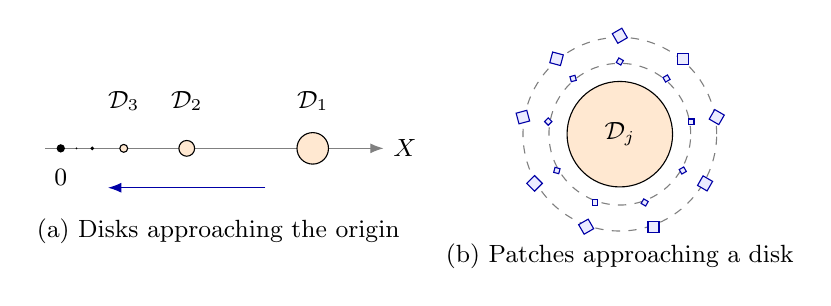
\begin{tikzpicture}[font=\small,>=Latex]
  \begin{scope}
    \draw[->,gray] (-.2,0)--(4.1,0) node[right,black] {\(X\)};
    \fill (0,0) circle (1.5pt) node[below=4pt] {\(0\)};
    \foreach \position/\radius/\disklabel in {3.2/.20/1,1.6/.10/2,.8/.05/3} {
      \draw[fill=orange!18] (\position,0) circle (\radius);
      \node[above=10pt] at (\position,0) {\(\mathcal D_{\disklabel}\)};
    }
    \fill (.4,0) circle (.025);
    \fill (.2,0) circle (.0125);
    \draw[->,blue!65!black] (2.6,-.50)--(.6,-.50);
    \node at (2,-1.05) {(a) Disks approaching the origin};
  \end{scope}
  \begin{scope}[shift={(7.1,.18)}]
    \draw[fill=orange!18] (0,0) circle (.67);
    \draw[gray,dashed] (0,0) circle (.90);
    \draw[gray,dashed] (0,0) circle (1.23);
    \foreach \angle/\innerrotation/\outerrotation in {
      10/0/60,50/30/0,90/60/30,130/15/75,170/45/15,
      210/75/45,250/0/30,290/60/0,330/30/60} {
      \begin{scope}[shift={(\angle:.923)},rotate=\innerrotation]
        \draw[blue!65!black,fill=blue!8] (-.033,-.033) rectangle (.033,.033);
      \end{scope}
      \begin{scope}[shift={(\angle:1.25)},rotate=\outerrotation]
        \draw[blue!65!black,fill=blue!8] (-.07,-.07) rectangle (.07,.07);
      \end{scope}
    }
    \node at (0,0) {\(\mathcal D_j\)};
    \node at (0,-1.55) {(b) Patches approaching a disk};
  \end{scope}
\end{tikzpicture}
\caption{The two accumulation levels, schematically and not to scale.
The disks in (a) are disjoint and avoid the origin. In (b), disjoint
full patches occupy successive annuli outside one disk. Only a few
patches and annuli are shown. Patch orientations are independent of
their positions around the disk; the actual construction approaches
every boundary point in every direction of a fixed finite rotation net.}
\label{fig:accumulation}
\end{figure}


Now prescribe \(K_0\). In each \(\mathcal D_j\) choose a smooth
negative bump, strictly negative throughout the disk and flat on
its boundary. In each patch choose a smooth bump supported in
\(\Phi_n((-4,4)^2)\), equal on a neighborhood of
\(\Phi_n([-3,3]^2)\) to
\begin{equation}\label{eq:patch-K0}
K_0(\Phi_n(x,y))=\kappa_n(x^2-h(y)),\qquad \kappa_n>0.
\end{equation}
The amplitudes of all disk and patch bumps can be chosen so that
their sum is smooth and \(\norm{K_0}_\infty\le10^{-3}\).
Here is a precise choice. Enumerate the unscaled, globally smooth
bump profiles, extended by zero, as \(k_n\). Choose positive
numbers \(\epsilon_n\) such that
\[
\norm{\epsilon_nk_n}_{C^m}\le10^{-3}2^{-n}
\qquad (0\le m\le n).
\]
There are only finitely many restrictions at stage \(n\).
For each fixed \(m\), the resulting series of derivatives has
a uniformly summable tail. Its sum is \(C^\infty\), including
on all accumulation sets. Disjointness of the supports preserves
the strict negativity inside each disk and the exact profiles
\eqref{eq:patch-K0}. Every summand is flat at each disk-boundary
point at which its support can accumulate, so
\[
K_0=0\qquad\text{on }\partial\mathcal D_j
\]
for every \(j\).

Apply \Cref{lem:prescribe} to obtain \(\bar g\).
For each patch, the actual pullback \(g_{0,n}=\Phi_n^*\bar g\)
has curvature
\[
K_{g_{0,n}}=K_{\bar g}\circ\Phi_n
=\kappa_n(x^2-h(y)).
\]
Indeed, in coefficient matrices,
\(g_{0,n}=\lambda_n^2R_n^T(\bar g\circ\Phi_n)R_n\);
curvature is a scalar under pullback.
This is a background metric of the kind required in
\Cref{sec:model}.

By \Cref{prop:patch}, choose a smooth tensor perturbation
\(\eta_n\) supported in the model box \(\mathcal P\) such that
\(g_{0,n}+\eta_n\) admits no admissible height.
Push \(\eta_n\) to the original coordinates and extend by zero,
obtaining \(\widehat\eta_n\).
The extension is smooth because its support is strictly inside
the full patch. In matrix notation the pushforward is
\[
\widehat\eta_n
=\lambda_n^{-2}R_n(\eta_n\circ\Phi_n^{-1})R_n^T.
\]
Consequently, for each ordinary derivative order \(m\),
\[
\norm{D^m\widehat\eta_n}_\infty
\le C_m\lambda_n^{-m-2}\norm{D^m\eta_n}_\infty,
\]
where \(C_m\) accounts only for the fixed-dimensional component
norms and rotation. The perturbation may be chosen arbitrarily
small in every prescribed finite collection of seminorms, so
these fixed scaling costs can be paid separately on each patch.
Require
\begin{equation}\label{eq:tensor-sum}
\norm{\widehat\eta_n}_{C^m}\le\epsilon\,2^{-n}
\qquad(0\le m\le n),
\end{equation}
where \(\epsilon>0\) is smaller than half a uniform lower
eigenvalue bound for \(\bar g\).
The metric
\begin{equation}\label{eq:final-metric}
g=\bar g+\sum_{n=1}^\infty\widehat\eta_n
\end{equation}
is therefore smooth and positive.
It retains the chosen patch obstruction on every patch:
all the other tensor perturbations vanish there.
Every tensor perturbation and all its derivatives vanish on
each closed disk. Uniform convergence of the derivative series
in \eqref{eq:tensor-sum} consequently preserves the background
metric jets on those disks and their boundaries. Thus
\begin{equation}\label{eq:disk-curvature}
K_g<0\text{ in }\mathcal D_j,\qquad
K_g=0\text{ on }\partial\mathcal D_j.
\end{equation}
This construction imposes no lower bound on the individual
\(\kappa_n\), \(\lambda_n\), or admissible Hessian separations.

\subsection{The boundary obstruction}

The following graph observation is also used in the geometric
construction of \cite[Section~2, Step~3]{NY2002}. We include its short proof.

\begin{lemma}[A negatively curved disk]\label{lem:disk}
Suppose a smooth metric on a neighborhood of a closed disk
has negative curvature in the disk and zero curvature on its
boundary. If an isometric immersion of this neighborhood is
a graph over a plane, its second fundamental form is nonzero
at some boundary point. At that point it has rank one.
\end{lemma}

\begin{proof}
Let \(u\) be the graph function and let \(\Omega\) be the planar
projection of the disk. This is a bounded domain with connected
smooth boundary, and \(u\) is smooth on a neighborhood of
\(\overline\Omega\). Suppose the second fundamental form vanishes
at every boundary point. The graph formula
\[
\II_{ij}=\frac{u_{ij}}{\sqrt{1+\abs{Du}^2}}
\]
then gives \(D^2u=0\) along \(\partial\Omega\). Differentiation
along this connected curve shows that \(Du\) is a fixed vector
\(a\) there. Hence \(u=a\cdot x+c\) on the boundary for a constant
\(c\).

The function \(v=u-a\cdot x-c\) is zero on \(\partial\Omega\)
and has
\[
\det D^2v=\det D^2u<0\qquad\text{in }\Omega.
\]
It cannot vanish identically. If it is nonzero, compactness
gives either a positive interior maximum or a negative interior
minimum. Its Hessian is semidefinite there, with nonnegative
determinant, a contradiction.
Thus the second fundamental form is nonzero at some boundary
point. The Gauss equation and zero boundary curvature make
its determinant zero, so its rank is one.
\end{proof}

\begin{proof}[Proof of Theorem~A]
Use the metric \eqref{eq:final-metric}.
Suppose that a neighborhood of the origin admits a smooth
isometric immersion \(F\) into \(\R^3\).
Projection onto the tangent plane at \(F(0)\) is a local
diffeomorphism. After restricting the domain, the immersion
is a graph and the projection is a diffeomorphism onto a
planar open set. Choose \(j\) so large that
\(\overline{\mathcal D_j}\) lies in this restricted domain.
By \eqref{eq:disk-curvature} and \Cref{lem:disk}, there is
\(b\in\partial\mathcal D_j\) where \(\II\) is nonzero and
has rank one.

Let \(e\) be the fixed unit normal at \(F(b)\), and set
\(z=\langle F,e\rangle\). By \Cref{lem:height}, the covariant
Hessian \(H\) is nonzero and rank one at \(b\), while \(dz(b)=0\).
In particular \(1-\abs{dz}_g^2>0\) nearby.

Regard \(H(b)\) as a symmetric form in the fixed \(X,Y\)
parameter plane. Choose a rotation in our finite net whose
first-axis line makes angle less than \(1/1000\) with its
kernel. In that rotated parameter frame, a rank-one form
has
\[
H_{yy}(b)\ne0,\qquad
\abs{H_{xy}(b)/H_{yy}(b)}
=\abs{\tan\alpha}<1/100,
\]
where \(\alpha\) is the angular error.
Continuity gives the same strict inequalities in a
neighborhood of \(b\).

There are full patches of this orientation converging to \(b\).
One such patch lies wholly in that neighborhood and in the
domain of \(F\). Its common dilation of the two axes multiplies
all Hessian entries by the same positive factor, leaving their
ratio unchanged. In model coordinates the pulled-back height
is therefore smooth on a neighborhood of \(S\), has \(E>0\),
\(H_{yy}\ne0\), and \(\abs q\le1/100\) throughout \(S\).
It satisfies the Darboux equation by \Cref{lem:height}.
It is an admissible height for a metric chosen to have none,
contradicting \Cref{prop:patch}.

Thus no neighborhood of the origin admits the asserted smooth
isometric immersion. The open square with the smooth positive
metric \(g\) is the required Riemannian surface.
\end{proof}

\begin{corollary}[Euclidean Taylor jet]\label{cor:flat-jet}
The metric in Theorem~A can be chosen so that, in the coordinates
\(X,Y\),
\[
\partial^\alpha(g_{ij}-\delta_{ij})(0)=0
\qquad
\text{for every multi-index }\alpha\in\mathbb N_0^2
\text{ and }i,j\in\{1,2\}.
\]
Thus smooth local isometric realizability is not determined by
the full Taylor jet of the metric at the base point.
\end{corollary}

\begin{proof}
Every individual curvature bump and every tensor
\(\widehat\eta_n\) vanishes on a neighborhood of the origin.
The uniform convergence of each derivative series therefore gives
\[
\partial^\alpha K_0(0)=0,
\qquad
\partial^\alpha\Bigl(\sum_n\widehat\eta_n\Bigr)(0)=0
\]
for every multi-index \(\alpha\).
It remains to check the background metric
\(\bar g=\dd X^2+f^2\dd Y^2\).
The initial conditions in \eqref{eq:prescribe-ode} give
\(\partial_X^a\partial_Y^b(f-1)(0)=0\) for \(a=0,1\)
and every \(b\ge0\). For \(a\ge2\), the same equation yields
\[
\partial_X^a\partial_Y^b(f-1)(0)
=-\partial_X^{a-2}\partial_Y^b(K_0f)(0)=0,
\]
since every term in the Leibniz expansion contains a derivative
of \(K_0\) at the origin. Hence \(f-1\), and therefore
\(\bar g_{ij}-\delta_{ij}\), has zero derivatives of every order
there. Adding the tensor series preserves this property.
The Euclidean metric itself admits an isometric immersion into
\(\R^3\), whereas the constructed metric does not on any
neighborhood of the origin.
\end{proof}


\bibliographystyle{plain}
\bibliography{references}
\end{document}
